\documentclass{article}
\usepackage{graphicx, color}


\setlength{\textwidth}{6.5in}
\setlength{\textheight}{8.0in}
\setlength{\oddsidemargin}{0in}
\setlength{\evensidemargin}{0in}
\setlength{\parskip}{2ex}
\setlength{\parindent}{0in}

%To display answers, replace "white" with "red" here;
\newcommand{\answer}[1]{\color{white}#1}

\begin{document}
\pagestyle{myheadings}\markright{
CU Boulder \hspace{0.5in} MATH 2510 - Introduction to Statistics }

\begin{center}
\textbf{\underbar{In-class Worksheet 2}}
\end{center}

\begin{enumerate}

\item Shown here is a histogram displaying the mileage, in miles per gallon, for a random selection of passenger cars. 

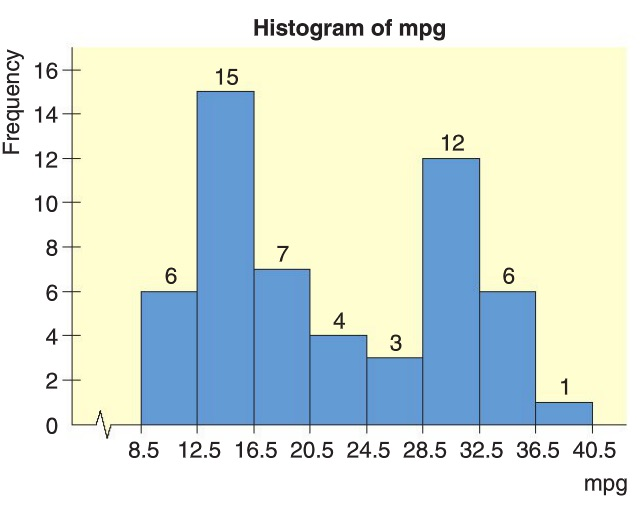
\includegraphics[scale=0.25]{WS2_MPGall.jpg} 

	\begin{enumerate}
	\item How many total data values were used to create this histogram?
	
	{\answer{Summing the numbers sitting at the top of each bar in the histogram (which represent the frequencies of data in each category), $6+15+7+4+3+12+6+1 = 54$}} 
	
	\item What is the most common range of  ``miles per gallon" for a passenger cars in this sample?

	{\answer{The interval from $12.5$ to $16.5$ contains 15 cars which is the highest frequency.}} 

	\item Describe the shape of this distribution.  (Mound-shape symmetrical, Uniform, Skewed left, Skewed right, Bimodal).
	
	{\answer{This is a bimodal distribution.}} 
	
	\item Curious about the bimodal shape of the distribution above (Is this consistent with your answer just above?), Jose did some research and found that this distribution included both city and highway mileage for each car in the sample.  Looking at the raw data, Jose discovered the following histogram displays the the City Mileage for the cars in the sample. 
	
	Use the information from the two histograms to draw a histogram for the Highway Mileage. (Use class boundaries consistent with the two histograms already shown.)
	
	\parbox[c]{2in}{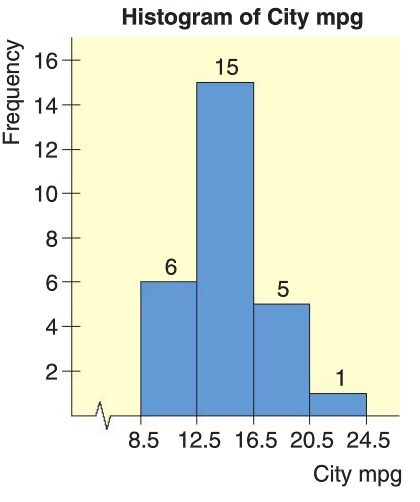
\includegraphics[scale=0.25]{WS2_MPGcity.jpg}}
	
	{\answer{\parbox[b][4em][t]{3in}{Draw a histogram with the same axes as the original histogram and the following frequencies 
	\begin{tabular}{c|c}
	Class & Frequency \\
	\hline
	$8.5-12.5$ & 0 \\
	$12.5-16.5$ & 0 \\
	$16.5-20.5$ & 2 \\
	$20.5-24.5$ & 3 \\
	$24.5-28.5$ & 3 \\
	$28.5-32.5$ & 12 \\
	$32.5-36.5$ & 6 \\
	$36.5-40.5$ & 1 \\
	\end{tabular}}}}  \\

	\end{enumerate}


\item Shown here is the relative frequency histogram (from D2L) of the overall course totals for MATH 1081 in Spring 2013 (600 students). 

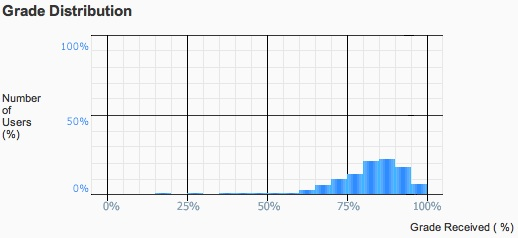
\includegraphics[scale=0.5]{WS2_1081Grades.jpg} 

	\begin{enumerate}
	\item Describe the shape of this distribution.  (Mound-shape symmetrical, Uniform, Skewed left, Skewed right, Bimodal).
	
	{\answer{This distribution is mound-shaped, but left-skewed.}} 
	
	\item Approximate the number of students that earned a 80\% or higher in the class.
	
	{\answer{The students that scored 80\% or higher are shown in the four rightmost bars.  Those fours bars represent about $21\%+22\%+19\%+8\%=70\%$ or $420$ students.}} 
	
	\end{enumerate}

\item Use the following figure to answer the questions below.

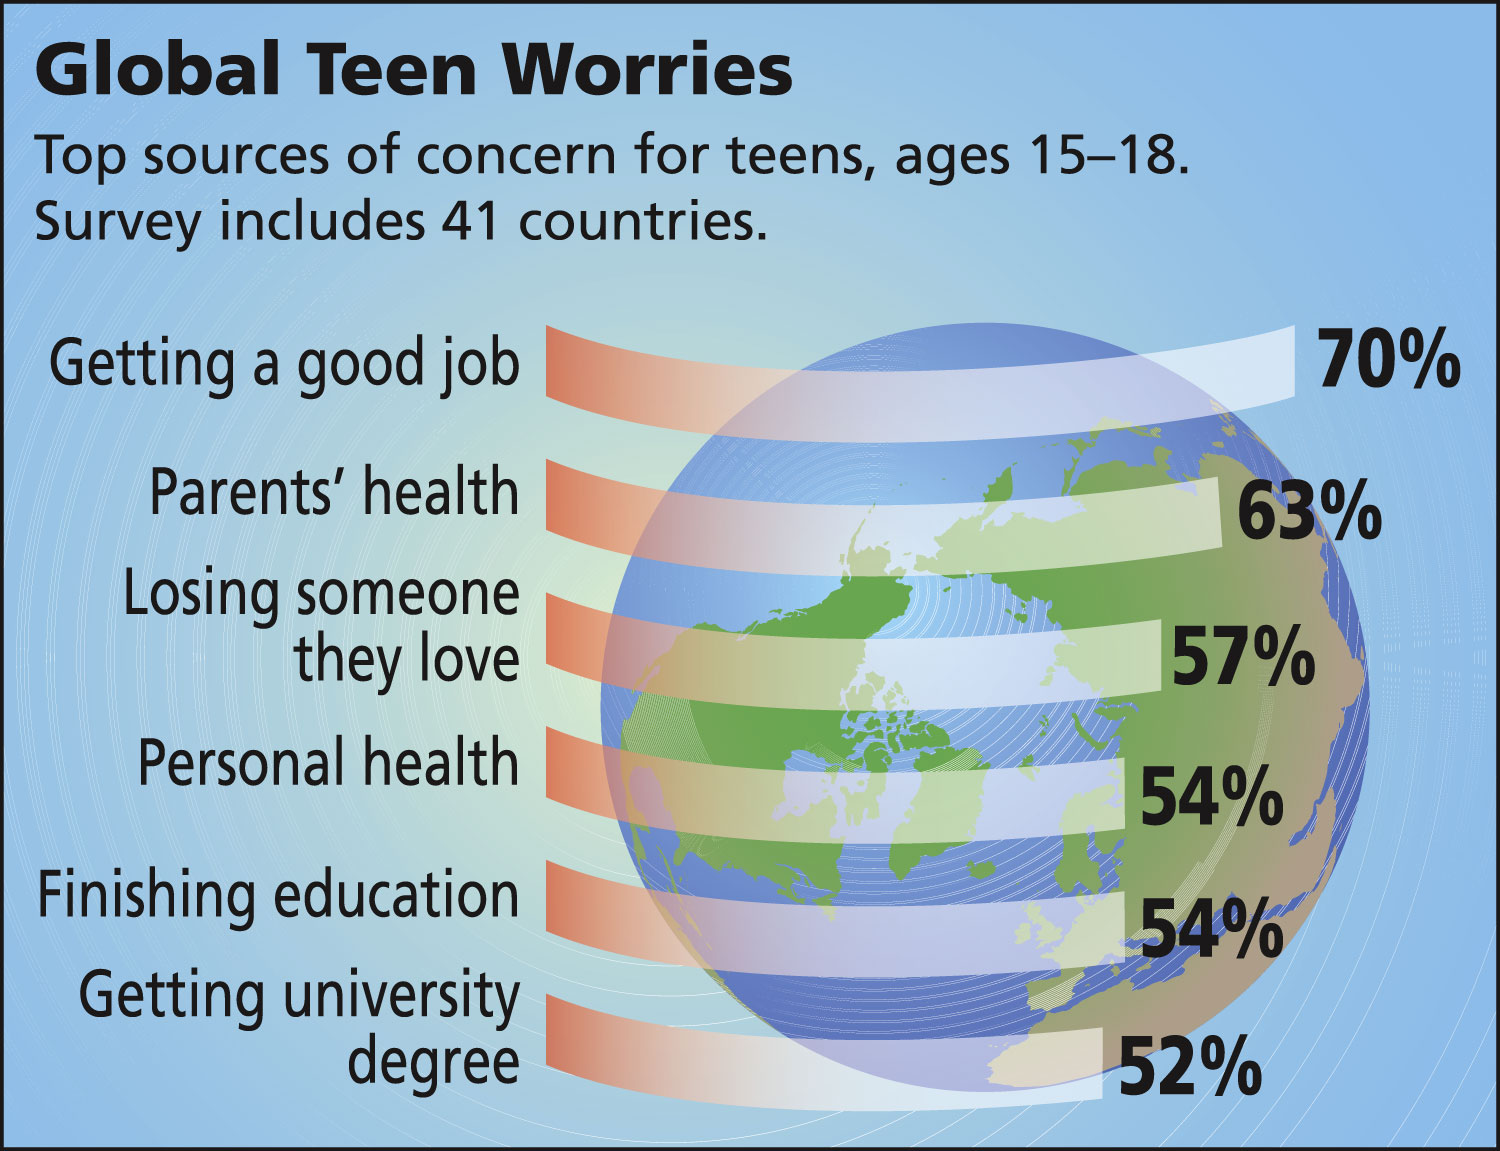
\includegraphics[scale=0.1]{WS2_Bar.jpg} 

	\begin{enumerate}
	\item Is this a bar graph?  Why or why not? 
	
	{\answer{This is a bar graph, since it uses the lengths of the bars to represent the (relative) frequency of occurrence of each data value.  It could be improved by using a scaled horizontal axis.}} 
	
	\item Could the same information be displayed in a Pareto chart?  Explain.
	
	{\answer{The graph shown is essentially already a Pareto chart because the (relative) frequencies of occurrence of each data value are being displayed in decreasing order.  Just rotate the figure 90-degrees counter-clockwise to make the presentation with vertical bars.}} 
	
	\item Could the same information be displayed in a circle graph?  Explain.
	
	{\answer{This data could not be display in a circle graph, since the percentages do not represent the parts of a whole.}}
	
	\end{enumerate}
	
\newpage
	
\item Without proper context and labels, ogives and time-series graphs can look very similar.  Given here are two different graphs (both intentionally lacking labels and context).  In {\em each} case determine if the graph can possibly represent an ogive and if it can possibly represent a time-series graph.  Explain.  
(Note, I am not saying that one IS an ogive and one IS a time-series.  For each graph decide if either, both, or neither option of ``ogive" or ``time-series" is possible and explain why or why not.)

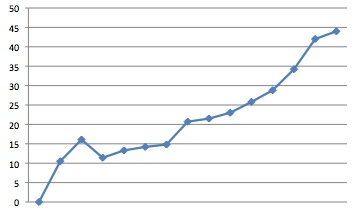
\includegraphics[scale=0.4]{WS2_Time.jpg} \hspace{4cm}
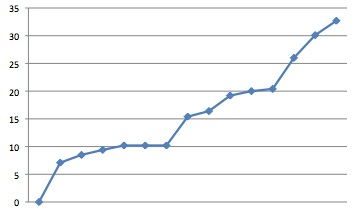
\includegraphics[scale=0.4]{WS2_Ogive.jpg}

	{\answer{\parbox[t]{2.0in}{In this case, there is a decrease in values from left to right, so this could not be an ogive, where the values of cumulative, hence always non-decreasing.  It could be a time-series graph.}
	\hspace{4cm} \parbox[t]{2.0in}{Since the data is always non-decreasing (from left to right), this could be both ogive and a time-series graph.}}} 


\item Using a {\em back-to-back} stem-and-leaf display, separate sets of data can more easily be compared.  Consider the following display for Midterm scores for two different sections of the same class.

\begin{center}
	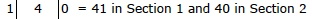
\includegraphics[scale=0.5]{WS2_StemLabel.jpg}
	
	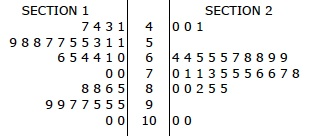
\includegraphics[scale=0.5]{WS2_Stem.jpg} 
\end{center}	

	\begin{enumerate}
	\item How many students took the Midterm in each section?
	
	{\answer{Section 1: 35 students; Section 2: 31 students}} 
	
	\item What are the highest and lowest scores earned in Section 1?  in Section 2?
	
	{\answer{Section 1: The highest score is 100.  The lowest score is 41. 
	Section 2:  The highest score is 100.  The lowest score is 40.}} 
	
	\item What is the score with the highest frequency of occurrence in Section 1?  in Section 2?
	
	{\answer{Section 1: The score with highest frequency is 95, with 3 occurrences. 
	Section 2:  The scores with highest frequency are 65 and 75, both with 3 occurrences.}} 
	
	\item Which section displays a more {\em consistent} understanding of the material?  Explain.
	
	{\answer{Section 2 shows 26 out the 31 students hovering in the interval of scores 64 to 85, where Section 1 is more spread out...not as notable of a {\em consistent} grouping.}} 
	
	\item Which section displays a {\em better} understanding of the material?  Explain.
	
	{\answer{Without computing anything, it may look as though Section 1 may have a higher average, since there are more scores above 90. On the other hand, section 1 also as more scores below 60. So it may be difficult to decide which class is ``better''. In fact, section 1 has a mean of $\approx 70.66$ and section 2 has a mean of $\approx 71.42$. So if we define ``better'' to be the higher average, then the answer is section 2. But we don't need to define better like this...}}
	\end{enumerate}
	
\end{enumerate}

\vfill

\end{document}

